\documentclass[12pt]{article}
\usepackage{fullpage}
\usepackage{epsf}
\usepackage{url}

\newtheorem{definition}{Definition}
\newtheorem{question}{Question}
\newtheorem{property}{Property}
\newtheorem{proof}{\em Proof}
\newtheorem{derivation}{\em Sketch}
\newtheorem{notation}{Notation}

\newcommand{\comment}[1]{}
\newcommand{\VS}{\mbox{\it VS}}
\newcommand{\WM}{\mbox{\it WM}}
\newcommand{\PCONJ}{\mbox{\it PCONJ}}
\newcommand{\kDNF}{\mbox{\it kDNF}}
\newcommand{\PDISJ}{\mbox{\it PDISJ}}
\newcommand{\DTrt}{\mbox{\it DT}_{r2}}
\newcommand{\DTs}{\mbox{\it DT}_s}
\newcommand{\PP}{{\rm P}}
\newcommand{\EE}{{\rm E}}
\newcommand{\PX}{\PP_{\!\scriptscriptstyle\! X}}
\newcommand{\PXY}{\PP_{\!\scriptscriptstyle\! X\!Y}}
\newcommand{\PYX}{\PP_{\!\scriptscriptstyle\! Y\!|\!X}}
\newcommand{\PYx}{\PP_{\!\scriptscriptstyle\! Y\!|x}}
\newcommand{\seq}[1]{\langle{#1}\rangle}
\newcommand{\RR}{I\!\!R}
\newcommand{\NN}{I\!\!N}
\newcommand{\argmin}{\arg\!\min}
\newcommand{\argmax}{\arg\!\max}
\newcommand{\eg}{{\em e.g.},\ }
\newcommand{\Eg}{{\em E.g.},\ }
\newcommand{\ie}{{\em i.e.},\ }
\newcommand{\Ie}{{\em I.e.},\ }
\newcommand{\cf}{{\em cf.}\ }
\newcommand{\etc}{{\em etc}}
\newcommand{\aka}{{\em a.k.a.}}
\newcommand{\vardef}{\stackrel{\triangle}{=}}
\def\norm [#1]{{\| #1 \|}}
\newcommand{\sign}{\mbox{\rm sign}}
\newcommand{\err}{\mbox{\rm err}}
\newcommand{\rank}{\mbox{\rm rank}}
\newcommand{\cond}{\mbox{\rm cond}}
\newcommand{\vect}{\mbox{\rm vec}}
\newcommand{\tr}{\mbox{\rm tr}}
\newcommand{\set}[1]{{\{#1\}}}
\newcommand{\tnorm}[2]{\|{#1}\|_{#2}}
\newcommand{\normdot}{{\mbox{$\|\!\cdot\!\|$}}}

%\newcommand{\makevector}[1]{{\tilde{#1}}}
\newcommand{\makevector}[1]{{\bf #1}}
\newcommand{\fvec}{{\makevector{f}}}
\newcommand{\evec}{{\makevector{e}}}
\newcommand{\bvec}{{\makevector{b}}}
\newcommand{\rvec}{{\makevector{r}}}
\newcommand{\dvec}{{\makevector{d}}}
\newcommand{\xvec}{{\makevector{x}}}
\newcommand{\qvec}{{\makevector{q}}}
\newcommand{\yvec}{{\makevector{y}}}
\newcommand{\mvec}{{\makevector{m}}}
\newcommand{\vvec}{{\makevector{v}}}
\newcommand{\zvec}{{\makevector{z}}}
\newcommand{\avec}{{\makevector{a}}}
\newcommand{\wvec}{{\makevector{w}}}
\newcommand{\cvec}{{\makevector{c}}}
\newcommand{\Xvec}{{\makevector{X}}}
\newcommand{\Fvec}{{\makevector{F}}}
\newcommand{\Avec}{{\makevector{A}}}
\newcommand{\Bvec}{{\makevector{B}}}
\newcommand{\Hvec}{{\makevector{H}}}
\newcommand{\Lvec}{{\makevector{L}}}
\newcommand{\Mvec}{{\makevector{M}}}
\newcommand{\Nvec}{{\makevector{N}}}
\newcommand{\Vvec}{{\makevector{V}}}
\newcommand{\Uvec}{{\makevector{U}}}
\newcommand{\Ivec}{{\makevector{I}}}
\newcommand{\Ovec}{{\makevector{O}}}
\newcommand{\smallxvec}{{\scriptsize\mathbf x}}
\newcommand{\alphavec}{\mbox{\boldmath $\alpha$}}
\newcommand{\betavec}{\mbox{\boldmath $\beta$}}
\newcommand{\muvec}{\mbox{\boldmath $\mu$}}
\newcommand{\phivec}{{\mbox{\boldmath $\phi$}}}
\newcommand{\lambdavec}{\mbox{\boldmath $\lambda$}}
\newcommand{\Lambdavec}{\mbox{\boldmath $\Lambda$}}
\newcommand{\Sigmavec}{\mbox{\boldmath $\Sigma$}}
\newcommand{\yy}{{\tt y}}
\newcommand{\uu}{{\tt u}}
\newcommand{\zerovec}{{\makevector{0}}}
\newcommand{\smallzerovec}{{\scriptsize\bf 0}}
\newcommand{\smallonevec}{{\scriptsize\bf 1}}
\newcommand{\onevec}{{\makevector{1}}}
\newcommand{\smallbetavec}{\mbox{\scriptsize\boldmath $\beta$}}
\newcommand{\smallmuvec}{\mbox{\scriptsize\boldmath $\mu$}}


\begin{document}

\noindent
{\Large\bf AUCSC 460 -- Artificial Intelligence}

\vspace*{1\baselineskip}

\noindent
{\large\bf Assignment 4: Classification Analysis}

\vspace*{1\baselineskip}

\noindent
Winter 2016\\
Department of Science\\
University of Alberta, Augustana Faculty

\vspace*{1.75\baselineskip}
\hrule

\vspace*{0.75\baselineskip}

\noindent
{\bf Due}: through eClass, {\em Monday, April 4}\\
{\bf Worth}: 25\% of final grade
\\
{\bf Instructor}: Anna Koop, HB 1-31, akoop@ualberta.ca

\vspace*{0.75\baselineskip}

\hrule

\vspace*{1\baselineskip}

\noindent
{\bf Note}
Please submit your assignment through eclass. Some questions require you to write small programs,
however for the written questions please format your answers
in a single {\em pdf\/} file.
Submit all required documents in a zip or tar archive.


\vspace*{1\baselineskip}

\hrule

\section{Using Weka}
You will be using Weka to analyze various classification methods on two data sets: the MNIST hand-written digit set and a spam email corpus. You will be comparing different learning algorithms, investigating the effect of parameter settings, and exploring feature generation possibilities.

%%%%%%%%%%%%
\section{Classification Comparison \rm(--12\%)}
MNIST arff files can be downloaded from here: \url{http://www.cs.ubc.ca/labs/beta/Projects/autoweka/datasets/mnist.zip}.

Load the MNIST data set into Weka and choose two classification algorithms. You may choose any algorithms, but you must know how they work. Run a series of experiments. Be sure to find the parameter settings for each algorithm that work best for the data. Present the results and discuss.

\subsection{Understanding classifiers \rm(--5\%)}
How do they work? What optimization criteria do they use? 

\subsection{Evaluation \rm(--4\%)}
Which does a better job? For what definition of "better??

\subsection{Evaluation \rm(--4\%)}
What parameter settings are best and why do you think that is?

%\begin{figure}[bt]
%\caption{|
%\label{fig:}
%\centering
%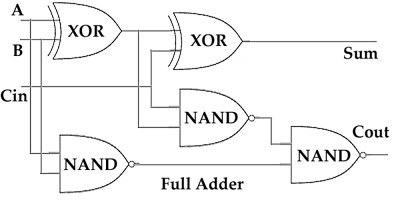
\includegraphics[width=.6\textwidth]{full_adder.png}
%\end{figure}


%%%%%%%%%%%%
\subsection{Understanding Features \rm(---13\%)}
Use the Spam Email corpus at this page: http://csmining.org/index.php/spam-email-datasets-.html. Note that the provided ExtractContent.py file runs in python 2.5 (your grader prefers to use python 3.x whenever possible).

Your first step is to load the Training data into Weka. This will require pre-processing to convert the directories of spam/ham email into a data format Weka recognizes.
\subsection{Basic Features \rm(--2\%)}
Explain the initial features (or attributes). 

\subsection{Feature transformations \rm(--5\%)}
What filters did yo apply to transform the data? Did you compute any new features? Did they work?

\subsection{Evaluation \rm(--5\%)}
What features worked best? Why do you think they did?

\subsection{Interaction of parameters and features \rm(--3\%)}
Did the same parameter setting seem to work best for all the feature sets you tried? You do not have to exhaustively compare, but do enough random samples to get a sense of whether this holds.
\end{document}
